In this section we will cover the constant optimization problem. A constant value can appear as a linear weight for a base function, or as a leaf. The following two functions clarify the difference.
\[
f(x) = \sin(\log(2, x))
\]
\[
g(x) = 3.14 sin(x) + 4.25 cos(x)
\]
In f the value of 2 is a constant value but not a linear weight to a base function. In g, 3.14 and 4.25 are both linear weights to sine and cosine respectively. In this work we focus on constant values that appear not as linear weights but as free constant arguments to base functions. Our tree encoding has a hidden linear weight for each node which could be optimized. When we refer to constant optimization, we are referring to the process of finding the optimal values of free constant arguments in the expression.

\subsection{Constant Optimization} \label{subconstantoptimization}
Selecting base functions is a combinatoric, discrete problem. Selecting the right constants to use is a continuous problem, that GP tries to solve with a combinatoric approach. There are several aspects to this issue, we will go over each individually and show our approach. 

\subsubsection{Restricting the search space}
From section \ref{searchspace} we know that the size of the constant set dominates the size of the search space. We intentionally restrict this set to [0,1]. This reduces the size of c from $2^{64}$ to $2^{23}$. This restriction in range does not prevent larger constants from being evolved. The algorithm will evolve subtrees combining base functions with constants in order to approximate the desired values. Selection [0,1] as the reduced range is a logical choice given that floating point numbers have the highest density in this range. Despite the significant reduction in size of c, it still dominates the search space size.

\subsubsection{Initialization revisited}
During initialization it is possible that a generated tree represents a constant expression. Such an expression is only a valid approximation if no feature influences Y, which is an unlikely edge case. A constant expression is of no use to the algorithm, but without measures to prevent or remove these they will still be formed. Typically such an expression will have a worse fitness value than non constant expressions, and will be eventually filtered out. Since detecting a constant expression is feasible in the worst case O(n) with n the number of nodes in the tree, a more efficient approach is preventing constant expressions from being generated. 

\paragraph{Constant expression detection}
An expression is a constant expression if all its children are constant expressions. As a base case, a leaf node is a constant expression if it is not a feature. This problem statement allows us to define a recursive algorithm to detect constant expressions. It should be noted that its complexity is O(n) only in the worst case, when the tree is a constant expression. Upon detecting a non constant subtree, the algorithm returns early without a full traversal. 

\paragraph{Preventing constant expressions}
Using the checking procedure in the initialization, a tree marked as a constant expression is not allowed in the initialization procedure.
It is still possible to create constant expressions by applying mutation and crossover. If the left subtree of a node is a constant expression, and the right is not, and this right is replaced by either mutation or crossover with a constant expression then the tree becomes a constant expression. The mutation operator will not generate constant subtrees, so this leaves only crossover. Our tool does not prevent constant expressions from forming in this way, the evaluation following crossover will filter out the constant expressions using evolutionary pressure.

\paragraph{Constant aliasing}
When we run the SR tool we do not know in advance which of our features influences the expected output. It is possible that some features have little or no effect whatsoever. If we have a feature z that has no effect on Y it is possible that, when the number of datapoints is low, the SR tool will start to use the values of z as a library of constant values. This unintended usage of z as a constant should be avoided at all costs as it will lead to a misleading surrogate model. In order to prevent this from occurring the values for any feature should be distinct and sampled so that they have sufficient distance between each other. Suppose we want to find a surrogate model for the function f:
\[
f(x, y, z) =\frac{sin(x) * cos(y)}{\ln(0.95)}
\]
If the range of x, y, and z is [0.9, 1] it is not difficult to see that the algorithm is likely to pick z to alias the desired constant value 0.95, instead of generating it. A resulting surrogate model could then be
\[
f'(x, y, z) =\frac{\sin(x) * \cos(y)}{\ln(z)}
\]
and have a reasonable fitness value but mislead a practitioner into assuming that z is a relevant feature. Since we have no information regarding f, not even if all features are needed, it is very hard to predict such behavior. The only way to mitigate this issue is to increase the number of datapoints and ensure that their distance is maximal. Increasing the range may help, but is often problem dependent and not under our control.

\subsubsection{Folding}\label{secconstfolding}

\paragraph{Constant subtree problem}
A tree can contain subtrees that represent constant expressions. This is an immediate effect of the GP algorithm trying to evolve the correct constant. This can lead to large subtrees that can be represented by a single node. Nodes used in such a constant subtree are not available for base functions. They waste memory and evaluation cost, without their presence the tree could become a fitter instance. 
There is a counterargument to be made here: parts of a constant subtree can help evolve constants faster than a pure random selection. It is therefore possible that folding such subtrees can lead to worse fitness values.

\paragraph{Constant subtree folding}
We can use a depth sensitive objective function to try to mitigate this effect, but a more direct approach is replacing the subtrees.
Using the previous constant expression detection technique we can collect all constant subtrees from a tree. We evaluate each subtree, and replace it with the constant value it represents. 
Constant folding requires an O(n) detection check, since the entire tree needs to be traversed. The folding operation itself is at worst O(n), if the entire tree is constant.

\begin{figure}
    \centering
    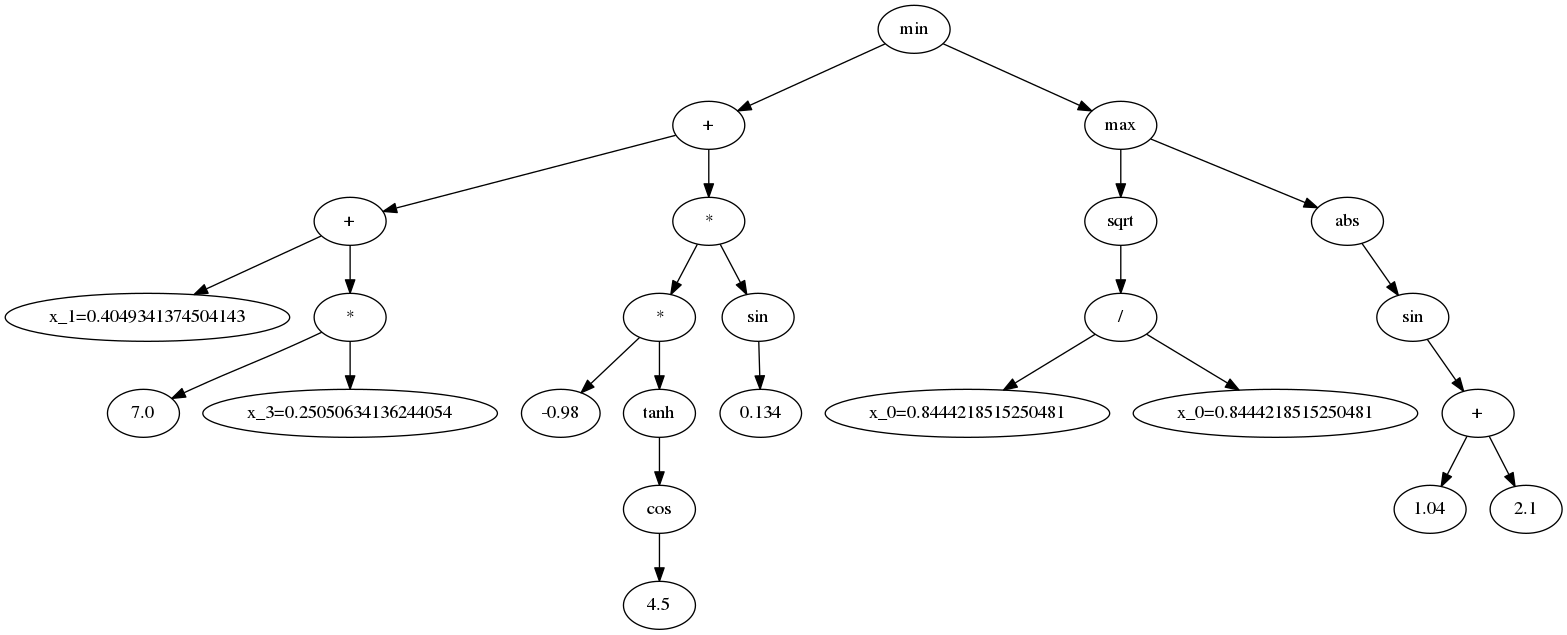
\includegraphics[width=\textwidth,height=\textheight,keepaspectratio]{figures/prefold.png}
    \caption{Tree before subtree folding.}
    \label{fig:prefold}
\end{figure}
\begin{figure}
    \centering
    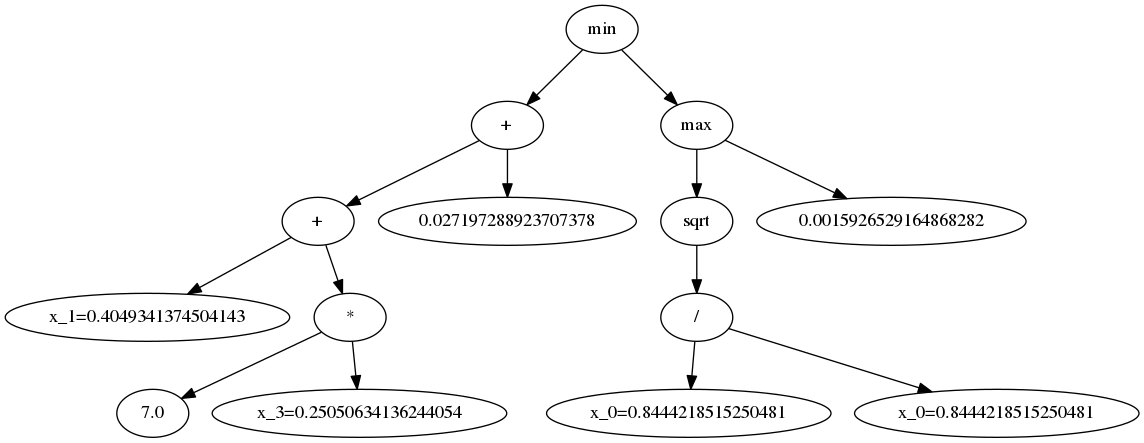
\includegraphics[width=\textwidth,height=\textheight,keepaspectratio]{figures/postfold.png}
    \caption{Tree after subtree folding.}
    \label{fig:postfold}
\end{figure}
\subparagraph{Analysis}
Constant folding leads to savings in nodes and possibly a reduction in depth. These savings can have an effect on the convergence as well. Mutation and crossover will no longer operate on constant subtrees, and the iterations and space in the tree that become available can be used to improve the fitness of the tree. These two advantages are intuitive and expected. There is also a counterintuitive disadvantage to constant folding. A constant subtree is the algorithm's attempt at evolving a single constant. In constant folding we assume that the subtree only holds the information needed to represent this single constant, and therefore is more efficiently represented by that single constant. This is not true. A constant subtree with depth d represents between d and $2^{d+1}-1$ constants. Each leaf is per definition a constant. Each internal node is the root of a constant subtree. Each of those represents a new constant, which is eventually combined to form the root of the largest constant subtree. Removing the entire subtree by folding it into a single constant can actually lead to worse fitness. To see this we need to look at constant subtrees as a set of discovered constants. The GP algorithm has 2 ways to generate a constant : crossover and mutation. Mutation will generate a subtree and replace an existing subtree in a tree. In order to generate a constant a constant subtree will need to be generated. This process is unaffected by folding. What is affected is when the mutation target node is a node in a constant subtree. Mutation is able to generate far more complex expressions than a single selection of a constant leaf node is able to do. If we apply constant folding mutation can only replace the existing constant with a new one. The probability of this new value having better fitness is lower compared to mutation the subtree that represents the constant. 
In crossover the effect is even stronger. The constant subtrees of a tree form a library of constants from which crossover can select and combine to form new values. Given the exponential number of constants represented by such a subtree it is clear that the expressive power of crossover without constant folding is greater than with constant folding applied. Constant folding is a trade-off between this expressive power and complexity. More importantly, constant folding is a necessity in order to optimize the constant values with a continuous optimizer. It reduces the dimensions of the optimization problem significantly.

\paragraph{Edge cases}
In Figure \ref{fig:postfold} we see the effect of applying the constant subtree folding. 
There are subtle edge cases that cannot be detected using the above method. Consider the tree representing the expression
\[
f(x) = \max(x, 4 + \sin(0.3)) 
\]
The subexpression 4 + sin(0.3) is detected and folded into the constant 4.26. 
We should not stop there, since f can still be a constant expression if $\forall i :  x_i < 4.26$. To verify this we need to evaluate f on all i datapoints. In contrast, the constant subtree detection code needs only 1 evaluation. In Figure \ref{fig:postfold} we see a similar case in the right subtree where the first value of $x_0$ the right subtree is indeed constant. 
Even if we should evaluate f for all i, this does not guarantee that f is indeed a constant expression. All this check proves is that for all i in the training data, f is constant. The testing data holds new values, for which f may or may not be constant. We conclude that this edge case cannot be prevented from occurring.
Another case occurs in expressions of the form 
\[
f(x, y) = \tan(y) * \sqrt{x/x}
\]
In this reduced example the node $\sqrt{x/x}$ is simply $\sqrt{1}$. Outside of this example, detecting such cases is non trivial. There is a clear benefit to do so, despite their low occurrence: if the domain of x includes 0 this tree is never generated because it leads to division by zero in a single datapoint. Discarding this expression is not needed, since $\sqrt{1}$ is a valid subexpression. One way to solve this is to use mathematical software to simplify the expressions and then convert them back to tree representations. Deciding to apply this step should be based on the cost versus benefit and the frequency of such occurrences. 

\paragraph{Conclusion}
Constant detection and folding mitigate some of the side effects of the constant optimization problem. We have discussed the advantages and the risks of applying constant folding. In general it is still advised to apply constant folding in order to constrain the excessive growth of trees in the population. In section \ref{subsecfoldingresults}
we will analyse the effect of constant folding.
Constant folding itself does not solve the constant optimization problem.
For this we need a continuous optimizer, an algorithm designed specifically to optimize real valued problems.

\subsection{Optimizers}

\paragraph{Hybridizing GP}
Using a real valued optimizer in combination with GP is a known solution \cite{GEDE, GPConst}.
Selecting an algorithm to combine with GP is a difficult question. To our knowledge there is no comparison made between optimizaton algorithms to find out which is a better fit to combine with GP. 

\paragraph{Problem statement}
Given a tree with k constant leaves, with all constant subtrees folded, we would like to find the most optimal values for those constants resulting in a better fitness. 
It is vital to perform the constant folding step before optimization takes place. Suppose a given tree has on average k constants, which after folding become j with j $<=$ k. Without folding the optimizer has to solve a k dimensional optimization problem, whereas after folding the problem is only j dimensional. The underlying approximation only has j dimensions, so this step is a necessity.

\paragraph{Initialization}
In most optimization problems the initial solution is not known, only the problem domain and an objective function. The problem we face here does have an initial solution, namely that generated by GP. Instead of choosing random points in the search space, we therefore opt by perturbing this initial solution. An immediate problem here is that the optimizer may simply converge on the initial solution. This risk can be high, given that GP already has evolved it as a suboptimal solution. 
The problem faced by the population initialization step \ref{subsubinvalidexpressions} reappears here. We could pick random values in the search space, but these are likely to generate invalid trees. A balance between exploration and exploitation is once again called for.

\paragraph{Domain}
Each tree instance has a completely different domain for each constant. We cannot guide the optimizer with domain specific knowledge. This also reflects in the choice of parameters for the optimizer, which will have to be suboptimal for specific problem instances, as we want them to work on the largest set of problems.

\paragraph{Comparison and configuration}
In order to keep the comparison between the algorithms fair they are each configured as similar as is possible. Since they are all population based, and given a maximum number of iterations, all three share these same parameter values. Each application of the algorithm has a significant cost in comparison with the main GP algorithm. In a single iteration with population p, the GP algorithm is likely to perform 2n evaluations (mutation and crossover). If we give the optimizer a population of m and q iterations, it will execute at most in the order of  m x q evaluations. Based on the optimal value for PSO \cite{PSO} we use a default population of 50. The iterations are set at 50. This means the cost of the optimizer will quickly dominate that of the main GP algorithm, depending on when and on what we apply it. We can apply the optimizer on each expression each iteration, only on a selection of the best expressions at each iteration, or only at the end of a phase on all, a selection, or only the best expressions. In our experiments we will show the effect of these choices on convergence.

\subsubsection{ABC}
Artificial Bee Colony \citep{ABC} is a relatively new nature inspired optimization algorithm. It is not limited to continuous optimization, and has even been used for symbolic regression itself \cite{ABCSR}. One of its key advantages over other algorithms is a lower parameter count. Optimal values for an optimization algorithm have a large impact on its convergence behavior, so much so that other optimizers can be required to find the parameters of an optimizer. With a small parameter set finding optimal values becomes easier. Finding optimal values for these parameters is quite often related to the problem domain, and as we have seen each instance here will have a new domain. ABC is good at exploration (thanks to the scouting phase) though sometimes lacking in exploitation. To resolve this ABC can be combined with more exploitative algorithms \citep{ABCPSO}.

\paragraph{Algorithm}
ABC is a population based algorithm, using 3 distinct phases per iteration. We will refrain from using the nature analogy in describing the algorithm as it can be confusing. The algorithm maintains a set of potential solutions and a population of particles. Each particle is either employed, onlooker, or scout. An employed particle perturbs a known solution, and if an improvement in fitness is obtained replaces the old solution. If this fails a preset number of iterations, the solution is discarded and a new one scouted. Scouting in this context is generating a new potential solution. After the employed phase the onlooking particles decide, based on a fitness weighted probability, which solutions should be further optimized. In contrast to the employed particles they swap out solutions each iteration, whereas an employed particle is linked to a single solution. Finally, exhausted solutions are replaced by scouted solutions.
\subparagraph{Initialization}
The algorithm initializes its solution set by perturbing it. Perturbation is done by multiplying each constant with a random number $\in [-1,1]$. Using the modified constants the tree recalculates its fitness value and updates the global best. Each instance records its best solution.
The original source, the expression tree that we wish to optimize, is retained as a solution, and not perturbed. This can lead to premature convergence if the algorithm is configured to focus too much on exploitation versus exploration.
 
\subparagraph{Modification}
In the employed stage, a solution x at time i is modified by combining it with another randomly chosen solution y. The choice for y is made with replacement, y $\neq$ x.
With k random $\in [0, \vert x \vert)$
\[   \left\{
\begin{array}{ll}
      x_{ij} = x_{ij} & j \neq k \\
      x_{ij} = y_{ij} & j = k \\
\end{array} 
\right.
\]
The employed particle tries to improve the current source. If the modification leads to an improved fitness value, the solution is updated. Note that only a strict improvement warrants an update, an equal fitness value will not lead to an update. 
The onlooker phase is executed next. Each onlooker is assigned a solution using roulette wheel selection.
For the set of solutions S we calculate fitness weights using:
\[
w_i = \frac{1}{1 + f_i} \forall i \in S 
\]
Optimization in CSRM is a fitness minimization process, hence the fraction. A list is built using a cumulative sum of these weights. From this a uniform random number selects a single value based on these weights. A smaller fitness value will have a relatively larger section of the list compared with a larger fitness value resulting in a fitness bias in selection. 
Once assigned to an onlooker, the same modification process used by the employed particle is applied. Since selection is done with replacement it is possible that a single highly fit value is modified more than once in an iteration. 
After the onlooker phase the algorithm checks in the scouting phase if any sources are exhausted. Exhaustion indicates that a solution cannot be improved for at least \textit{limit} modifications. Depending on the fitness value this limit can be reached faster for more fit values. There are several edge cases to consider here. Clearly this approach is beneficial if the exhausted solution has a poor fitness value. Improvement was impossible, so replacement is likely to improve the overall quality of the solution set by introducing new information. There is however the risk that the algorithm discards highly fit solutions that fail to be improved. Discarding such a solution is warranted if that solution is a local optimum, but by the very nature of the problem statement we cannot know this in advance. We could prohibit discarding the best solution, even if the improvement limit has been exceeded. This does not solve all edge cases. If ABC is used in a multimodal search, it is still possible that valid solutions are discarded. Compounding the problem is that an equality update is not used. In CSRM we implement a strict check, so it is possible that equivalent solutions are discarded. 
With s scouts and e exhausted solutions $min(s, e)$ solutions will be replaced with new solutions, generated using a normal distribution. In most optimization problems good starting positions are not known and thus a random point is selected. In our problem we already have a reasonably good solution, so we use this initial value as the mean of the normal distribution and generate values within 2 standard deviations. A configurable scaling factor is introduced, in our test problems we use 20. This value is a trade-off between exploration and an increasing probability for generating invalid solutions. The values chosen have a far greater range than those generated by the initialization process. We do not know the domain of our problem, nor do we have the computational resources to cover the entire floating point range. The initial value is already evolved as a fit solution to our problem. The probability that the true optimum is far beyond the range of our initial value is estimated as low, though we can never be sure of this. The scouted solution replaces the exhausted solution. In our problem statement this can lead to issues. There is no guarantee that the scouted solution is actually valid. As we have seen in the initialization problem \ref{subsubinvalidexpressions} this probability can be quite high. It is possible that an increasing part of the solutions are invalid. These will still be chosen to contribute in the modification step. It is unlikely though not impossible that they contribute to the convergence. In the worst case with enough iterations and a very small domain it is possible that the entire population is replaced with invalid solutions. In our implementation the values of the threshold regulating exhaustion are chosen such that this is unlikely to occur. One solution here is to apply the same generation loop used in the GP algorithm, which keeps generating solutions until a valid one is found. Given the already high cost in evaluations the optimizer introduces we have chosen not to use this here. This applies for all optimizers implemented in CSRM, not just ABC. Note that the same problem is present in the initialization step, although far less severe given the small perturbation applied there.

\subparagraph{Selection}
A solution is updated if the fitness value is improved. The new fitness weights for the roulette wheel selection are calculated and the global best is updated. Unlike PSO a solution is only updated if an improvement is measured. In contrast to DE, equal fitness values do not lead to an update. An equality update allows an optimization algorithm to cross zero gradient areas in the fitness landscape. The influence other solutions have on each other in ABC is not as great as in DE. From the modification stage we also observe that at most 2 dimensions per iteration per solution are modified. In PSO the entire position, in all dimensions, is updated. In DE this depends on the Cr parameter which we discuss in \ref{DEConfig}. This distinction can have a large impact on convergence. The balance sought here is influenced by the interdependence of the constants. The modifications made by the algorithm can be seen as a process trying to extract information about this dependency. Suppose we have k constants, of which 2 have a large effect on the result. Then it only makes sense to modify those 2 dimensions, modification in the others does not gain anything except noise. The problem becomes more difficult if those two are correlated. Modifying all dimensions will not guide our optimization process as clearly as modifying only those 2. Modifying only a single one of the 2, as in ABC, is too strict as we lose the information about the correlation.
We do not know in advance if our problem instances are separable or not. Related to this discussion, PSO can be sensitive to a bias along the axes of the dimensions \cite{PSOBias} with improvements suggested in recent work \cite{PSOBiasAlg}.


\paragraph{Cost}\label{abccost}
With a solution set of n, m employed, j scouts, i onlookers and k iterations we now look at the evaluation cost.
Initialization requires n evaluations. Each iteration we execute m evaluations in the employed phase, i evaluations in the onlooker phase and at most j evaluations in the scouting phase. With m, j and i all $<=$ to n we have per iteration at most 3n evaluations. With our configuration, listed below, this value will be at most 2n. This results in an evaluation complexity of n + k 2 n, or O(kn).

\paragraph{Configuration}
\begin{itemize}
\item limit = 0.75 * onlookers / 2 : If a solution can't be improved after this many iterations, it is marked exhausted and will be scouted for a new value. This limit is scaled by the number of dimensions per instance. 
\item population = 50 : This is the solution set, or set of sources.
\item onlookers = 25 : The number of onlookers, instances that will be assigned solutions to exploit based on fitness values. Setting this value to half that of the employed finds a balance between exploitation and evaluation cost.
\item employed = 50 : Instances that try to improve an assigned solution. If we use a value lower than the solution set we have to define an assignment procedure, which would mimick the onlooker phase. We therefore set the employed count equal to the size of the solutions set. 
\item scouts = 25 : This is a maximum value, up to this number are used to scout after a solution is exhausted. A higher scouting value leads to more exploration, a lower value favors exploitation. More exploration would result in the initialization problem dominating the runtime cost of the optimizer. 
\end{itemize}
This configuration is guided by the findings in \cite{ABC}.

\subsubsection{PSO}
Particle Swarm Optimization \cite{PSO} is one of the oldest population based metaheuristics. It consists of n particles that share information with each other about the global best solution.

\paragraph{Algorithm}
\subparagraph{Initialization}
Each particle is assigned an n dimensional position in the search space. A particle's position is updated using its velocity. This last is influenced by information from the global best and the local best. The concept of inertia is used to prevent velocity explosion \cite{PSOExplosion}.
Each particle is given a random location at start. In our application we already have an (sub)optimal solution, the constant values in the tree instances have been evolved by the GP algorithm. Rather than pick random values, we perturb the existing solution. This is a difficult trade-off. If the perturbation is not large enough the optimizer will simply converge on the known solution. If we perturb too much the risk for invalid solutions increases, rendering a large selection of the population invalid. We can initialize the population with n perturbed solutions or with n-1 with the initial value remaining intact. The n-1 solution is useful to test the algorithm, ideally the swarm will converge on the known best value. When applying the optimizer the n-perturbation approach is used, minimizing the risk for premature convergence.
CSRM multiplies each constant with a random value in [0,1].
Each particle is assigned a small but non-zero velocity. The reason for this is again avoiding premature convergence. Without this velocity all particles are immediately attracted to the first global best. While attraction to this value is desired, it should not dominate the population. The small value of the initial velocity once again reflects an empirically discovered balance between exploration and exploitation.
Each particle is assigned an inertiaweight.
This value is one approach to combat the velocity explosion problem, which we will cover next. 
Finally the global best is recorded. 


\subparagraph{Modification}\label{subppsomodification}
The algorithm updates all particles in sequence, then records the new global best.
Let d be the dimension of the problem, or in our case the number of constants in the tree to optimize.
The velocity v at iteration i of a particle is updated using:
\[
v_{i+1 j} = w_i * v_{ij} + C_1 * (p_{ij} - g_{ij}) * R_1 + C_2 * (p_{ij} - G_{ij}) * R_2 \forall j \in [0, d)
\]
with
\begin{itemize}
\item $v_i$ Current velocity
\item $p_i$ Current position (set of constant values)
\item $g_i$ Local best
\item $G_i$ Global best
\item $C_1$ Constant weight influencing the effect the local best has on the velocity.
\item $C_2$ Constant weight influencing the effect the global best has on the velocity.
\item $w_i$ Inertia weight simulating physical inertia.
\item $R_1$ Random value perturbing the effect the local best has on the velocity.
\item $R_2$ Random value perturbing the effect the global best has on the velocity.
\end{itemize}
Without the inertia weight PSO has issues with velocity explosion, the velocity has a tendency to increase to large values. This increases the distance between particles, but more importantly is far more likely to generate positions that are no longer inside the domain of one or more of the dimensions. Inertia weighting will dampen this effect. 
\\
The position is updated using :
\[
x_{i+1,j} = x_{ij} + v_{ij} \forall j \in [0, d)
\]
The $R_1$ and $R_2$ parameters make the modification stochastic, they introduce perturbations in the calculation. These changes have the benefit that they can break non optimal behavior resulting from the deterministic calculation. If there is a suboptimal best value (local or global) that leads to a too strong attraction and thus forcing premature convergence, we can with a certain probability escape from such a value by perturbing the velocity calculation. The C constants determine how strong the effects are of respectively the local best and the global best. This reflects the balance between exploration and exploitation respectively, where a particle is influenced more by its own information or that of the swarm.
After all particles are updated, the new global best is recorded for the next iteration.

\subparagraph{Selection}
An interesting difference with other the algorithms is that the position is always updated, whether it improves fitness or not. The local best records the best known position, but the particle is allowed to visit positions with lower fitness values. This allows it to escape local optima. The global best is obviously only updated with an improved value. The comparison is strict, meaning that only a better value can become the new global best. This may not seem significant, but allowing equality updates can actually benefit an optimization process. Allowing for equality updates allows the global best to move despite no apparent improvement in fitness,
it can traverse zero gradient areas in the fitness topology and thus escape local optima.

\paragraph{Cost}\label{psocost}
With a population size of n, the algorithm requires n fitness evaluations per iteration. The computational cost of updating the velocity and position is small given the evaluation cost of an expression tree over several datapoints. However, it is linear in d, the number of dimensions. If the tree increases in size, the number of constants can increase in the worst case exponentially. On average due to the construction algorithm we expect that half the leaves in the tree are constants. Given our discussion of the constant folding algorithm we know that a full binary tree is unlikely, so the number of constant nodes is equally unlikely to increase exponentially, but will nonetheless scale poorly.
In our implementation we will halt the algorithm if it cannot improve the global best after k/2 consecutive iterations, where k is the maximum number of iterations it can execute. The initialization stage adds another n evaluations, in addition to n per iteration. The total cost in fitness evaluations is therefore n(k+1), resulting in a worst case evaluation complexity of O(nk).

\paragraph{Configuration}
This overview gives the values of each parameter used in CSRM's PSO implementation.
\begin{itemize}
\item $C_1$ = 2 
\item $C_2$ = 2 : Setting both to 2 is recommended as the most generic approach \cite{PSOParameter}.
\item $w_i = \frac{1 + r}{2}$ with r random in [0,1] : In early implementations the inertia weight was kept constant \cite{PSOInertiaShi} There are a large number of strategies for an inertia weight. A dynamically decreasing inertia may improve convergence significantly. We opted for a random inertia weight as it has been shown \cite{PSOInertia} to lead to faster convergence for a generic problem set. Since our use case requires fast convergence on very limited iterations, this strategy is clearly favored.

\item $R_1, R_2$ r with r random in [0,1]
\item population = 50 : PSO is not sensitive to populations larger than this value, providing a robust default value. \cite{SwarmIntelligence}
\end{itemize}
CSRM's optimizer does not set constraints on the domain of each constant, these are unique to each problem instance. 
Finding the domain of a constant in the expression tree requires a domain analysis of the expression tree. Finding the exact domain is infeasible, given that some of the datapoints for features are unknown (e.g. validation or test date). It is therefore possible that a particle obtains values outside the valid domain of one or more constants, resulting in an invalid expression tree. This will result in the particle temporarily no longer contributing to the search process.

\subsubsection{DE}
Differential Evolution is a vector based optimization algorithm, or rather as the name implies, it operates by computing the difference between particles. 
\paragraph{Algorithm}
The algorithm has a population of n vectors, similar to the other algorithms it holds a linear set of values to optimize, one per dimension.  
\subparagraph{Initialization}
Similar to our approach in initialization PSO, we perturb a known (sub)optimal solution. A vector stores its current value, and the best value. 
\subparagraph{Modification}
Each iteration the algorithm processes all vectors. For each vector $\vec{v}$, three distinct randomly selected vectors are selected. From these 3 vectors a new 'mutated' vector is obtained:
\[
\vec{v} = \vec{w} + F (\vec{y} - \vec{z})
\]
With $\vec{w}$,$\vec{y}$,$\vec{z}$ randomly chosen and not equal to $\vec{v}$.\\
The selection occurs with replacement. Several selection schemes exists, and the size of the selection is equally configurable.
From this step the algorithm lends its name. The F factor influences the effect of the difference. 
Then we apply a crossover operation, using vectors x and v and probability parameter Cr.
We select a random index j with $ j \in [0, \vert x \vert)$. We then create a new vector u:
\[
u_i = k_i \forall i \in [0, \vert x \vert
\]
and $k_i$ equal to 
\[   \left\{
\begin{array}{ll}
      v_i & i = j \lor r < Cr \\
      x_i & i \neq j \land r \geq Cr \\
\end{array} 
\right.
\]
This is binomial crossover, another frequently used selection operation is exponential crossover.

\subparagraph{Selection}
For a given selected vector $\vec{v}$ and created vector $\vec{u}$ we now test if $\vec{v}$ is a better candidate than $\vec{u}$, in other words has a lower or equal fitness value. Note the distinction here with PSO, the equality test allows DE vectors to cross areas with a zero gradient. If f($\vec{u}) \leq  f(\vec{v})$ the vector is replaced with $\vec{u}$. The global and local best are updated as well. A difference with PSO is that a PSO particle changes regardless of fitness value, whereas in DE the modification is only committed if a better or equal fitness value is obtained. The first approach allows an optimization algorithm to break free from local optima. DE uses the random selection of other vectors to create a similar effect. If we use the landscape analogy, as long as at least one DE vector is outside a depression in the fitness topology, but all the others are converging to the suboptimal minimum, DE has a probability to escape a local optima. Unlike PSO DE (in our configuration) does not use the global best in its calculations, sharing of information is completely distributed over the vectors.
\paragraph{Cost}\label{decost}
For each vector 3 other vectors are used, or restated we create 2 new vectors. Similar to PSO these calculations have a complexity linear in d, the dimensionality of the problem. The fitness function is called once per iteration per vector. Compared to PSO we therefore have the exact same evaluation complexity of O(nk).

\paragraph{Configuration}\label{DEConfig}
CSRM uses a DE/rand/2/bin configuration. The DE/x/y/z notation reflects its main configuration, where x is the vector perturbed, y is the vectors used in the differential step and z is the crossover operation (binomial). This configuration is referenced \cite{DE} as one of the most competitive for multimodal problems with good convergence characteristics to the global optimum. Since we start from a probable local optimum the choice for a random vector instead of the global best vector also helps avoid premature convergence.
This overview gives the values of each parameter used in CSRM's DE implementation.
\begin{itemize}
\item F = 0.6 : F should be in [0.4, 1] Large F values favor exploration, whereas small F values favor exploitation. The value of 0.6 is reported as good starting value\citep{DESurveyLatest}. In our problem domain we already have a (sub) optimal solution which we wish to improve, so the risk of premature convergence is present, hence the small bias for exploration. 
\item Cr = 0.1 : The Cr values should be in [0,0.2] for separable functions, and [0.9, 1] for non separable functions. We cannot assume dependency between the constants, and therefore use a value of 0.1. This results in DE focussing along the axes of each dimension in its search trajectory. 
\end{itemize}
Compared to PSO DE has a low parameter count, optimal values for these parameters can be found in literature \cite{DESurveyLatest}. The population size should be t * d with t in [2, 10]. Since we do not know d in advance, and to keep the comparison fair we set the population at 50, allowing for optimal values for up to 25 dimensions (constants).
While DE has a small set of parameters, their effect is still quite pronounced. There exists implementations of DE that use self adapting parameters, but this is beyond our scope. It should be noted that CSRM's optimizer has a very small optimization budget (in evaluation cost) and each new problem has potentially new characteristics. We therefore chose for the most robust values and configuration.